\chapter{Datenmodell}
\liable{\cii}
An dieser Stelle wird die Umsetzung des in Abschnitt \ref{spec:model} 
beschriebenen vereinfachten Datenmodells detaillierter beschrieben. 
Dabei ist einmal die Umsetzung auf die Datenbank sowie die XML-Dateien und eine objektorientierte
Abbildung vonnöten.

\section{Datenbank}
Bei der Umsetzung des Datenmodells in ein Datenbankschema wird besonders auf kompakte Datenhaltung geachtet. 
Die Typenbezeichnungen sind leicht SQLITE-affin, könnten aber bei der Änderung des DBMS relativ einfach umgewandelt werden.
\subsection{Normalisierung} Um die angesprochene kompakte Speicherung der Daten zu erreichen,
wird die Struktur normalisiert \ref{req:Db:normalize}. \\ 
paragraph{Beschreibung:}
\begin{description}
	\item [metaData]
		In dieser Tabelle liegen alle statischen Teile einer Datei, 
		die sich nach dem ersten Herunterladen nicht mehr ändern können. 
		Pro im Archiv gespeicherter Datei kommt unabhängig von deren Version deshalb 
		immer nur \emph{ein} Eintrag in der Tabelle vor.
	\item [history]
		Die Tabelle history enthält alle Einträge einer Datei, die sich mit der Zeit ändern
		können. Somit kann es pro Datei mehrere Einträge geben, aber immer nur einen pro Version.
	\item [commitTag]
		Ein commitTag-Eintrag erfolgt immer beim Crawlen von Webseiten. Dabei kann ein
		commitTag die Versionsstände mehrerer Dateien beinthalten.
		Die commitTime ist dabei der Schlüssel um die Daten aus der Versionierung
		auschecken zu können.
		Ein commitTag gehört durch die aufgeteilte Versionierung (\ref{req:Ar:domainversion}) immer zu einer bestimmten Domain
	\item [domain]
		Um die im Verhältnis zu gespeicherten Dateien kleine Menge an Domainnamen kompakt zu speichern,
		werden diese in eine eigene Tabelle ausgelagert.
	\item [mimeType]
		Ein ähnliches Verhältnis wie bei den Domainnammen herrscht bei der Bezeichnung der mimeTypes.
		Deshalb wird dieser ebenfalls ausgelagert.
		Der mimeType wird unter anderem zum Herausfiltern von Dateien benötigt (\ref{req:Fi:testfilter}).
\end{description}
Tabellendiagramm \ref{dia:design:frontend:data:db} gibt einen graphischen Überblick.
\paragraph{Anmerkung:} Für TimeStamps wird ebenfalls das in \ref{spec:model} spezifizierte (XML-)Textformat
verwendet. Damit ist eine einfache Portierbarkeit zwischen XML, Java, Python und Datenbank am besten gewährleistet.

\begin{figure}[h]
	\centering
	\label{dia:design:frontend:data:db}
	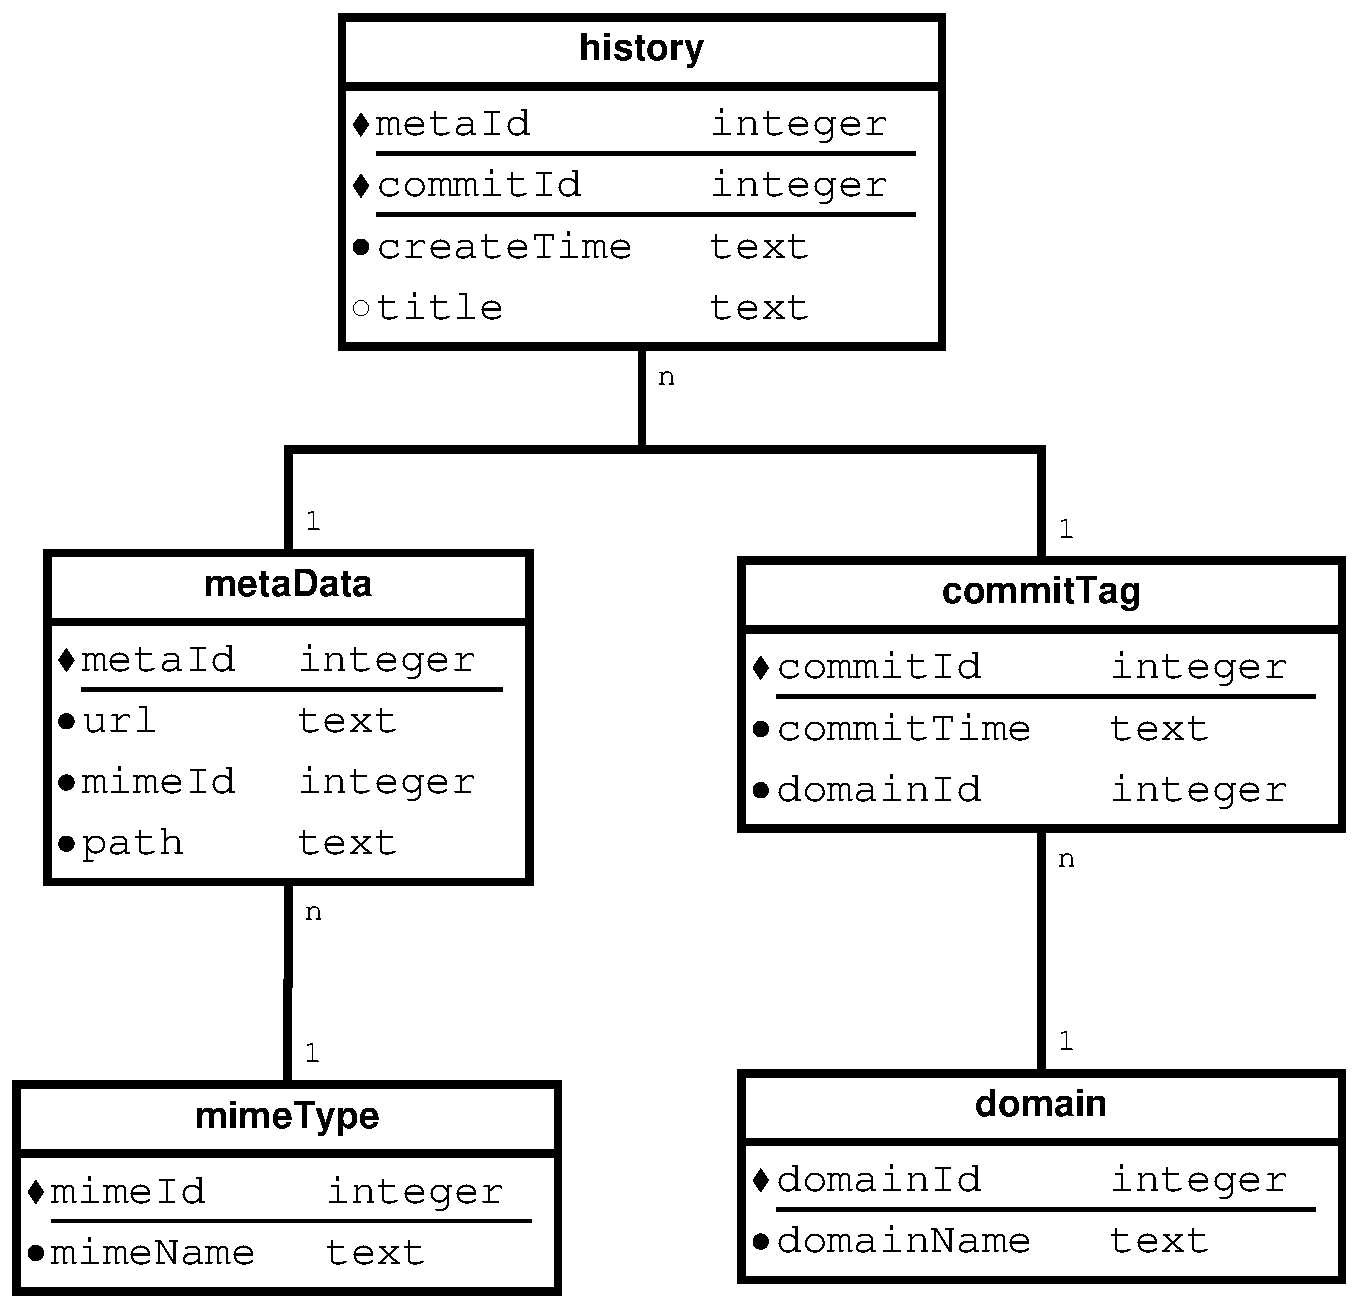
\includegraphics[width=0.6\textwidth]{design/data/db.eps}
	\caption{Datenbankdiagramm}
\end{figure}

\section{XML-Schema}
Folgendes Skripting des XML-Schemas (\ref{req:Xm:schema}) zeigt den Aufbau der XML-Datei:
\lstinputlisting[language=XML,basicstyle=\ttfamily\fontsize{8}{10}\selectfont]{../src/xml/file.xsd}
\subsection{Metadaten}
\ref{req:Xm:content:meta}
Um die Metadaten kompakter und besser lesbar zu gestalten, 
werden diese als Attribute ausgeführt. 
Dabei wird auch die 1:n-Beziehung von commitTag zu Metadaten berücksichtig:
Die commit-Daten bilden ein Unterelement von ,,meta'' und sind in diesm ebenfalls als
als Attribute enthalten.
Damit ist der commitTag auch leichter auslesbar.


Im Gegensatz zum DB-Schema erfassen die XML-Metadaten immer den gesamten Zustand innerhalb der zugehörigen Version (bzw. zu einem CommitTag), also redundant. 
\subsection{Daten}
\ref{req:Xm:content:data} \\
Das ,,data''-Element ist anfangs immer leer, kann aber durch Benutzer mittels der API-Schnittstellen 
um weitere Elemente (sog. DataElemente) erweitert.
Dabei ist auch das XSD-Schema entsprechend dem auskommentierten Template zu erweitern.
Der Name des umschließenden DataElements muss dabei einmalig sein.

Folgendes Listing zeigt ein Beispiel XML mit leerem data-Knoten:
\lstinputlisting[language=XML,basicstyle=\ttfamily\fontsize{8}{10}\selectfont]{../src/xml/example.xml}

\section{Klassen} \label{design:data:classes}
Diagramm \ref{dia:design:frontend:data:classes} zeigt die Umsetzung des Modells in Klassen.
Aufgrund der 1:n-Beziehung (siehe oben) von Metadaten und CommitTags sind die entsprechenden
Klassen auch getrennt.

Damit ist es auch möglich speicherintern CommitTags in Metadaten wiederzuverwenden.
Außerdem werden die CommitTags zur Benachrichtigung der Clients durch den Notifier benötigt
und ermöglichen ein effizienteres Auslesen aus der Datenbank.

Die TimeStamp-Klasse dient zur Vermittlung zwischen der textbasierten Speicherung von Datumswerten und der
programmierspracheninternen Darstellung z.B. java.util.Date.

Analog zu den XML-Daten enthält ein Metadatenobjekt immer den gesamten Zustand einer Datei zu einem CommitTag.

\begin{figure}[h]
	\centering
	\label{dia:design:frontend:data:classes}
	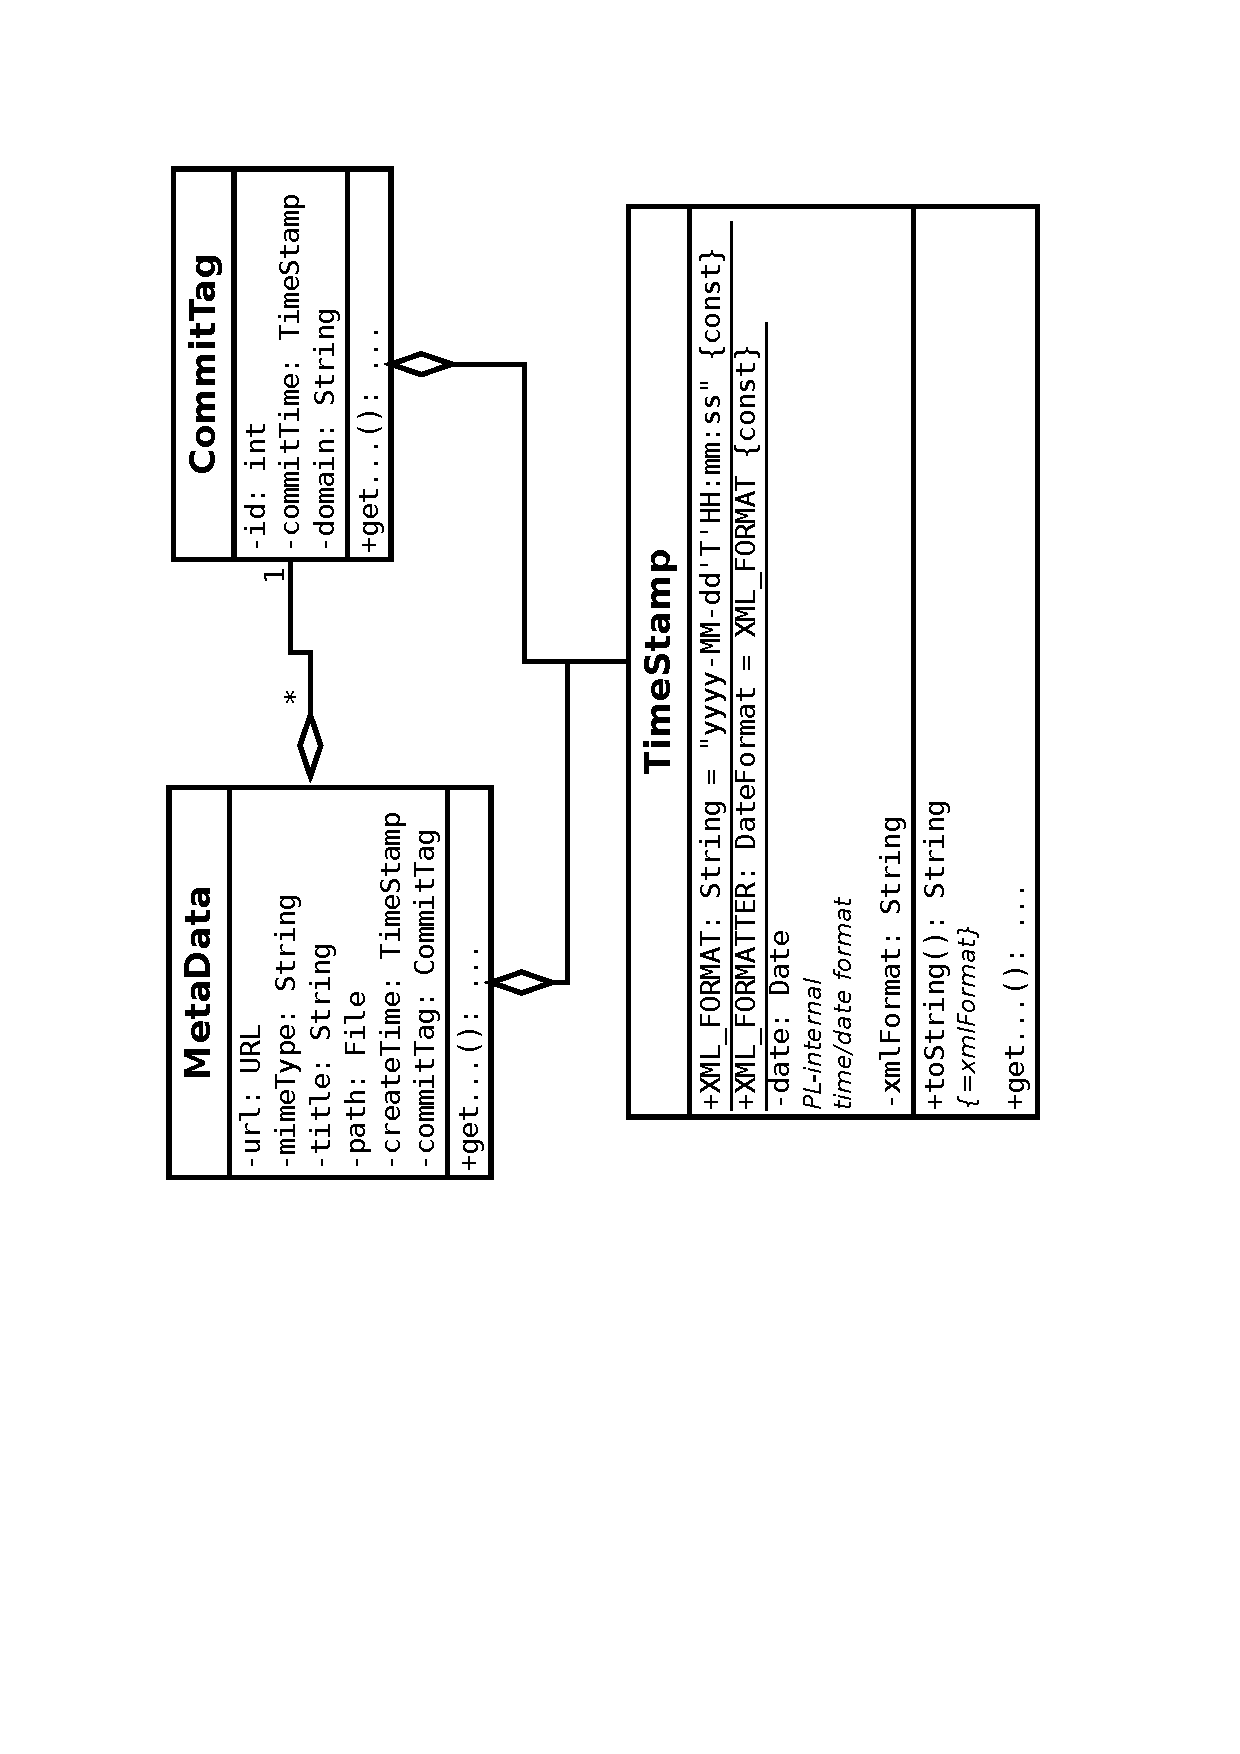
\includegraphics[width=0.7\textwidth, angle=270]{design/data/model.pdf}
	\caption{Datenbankdiagramm}
\end{figure}

